\textbf{f)} Tome 3 puntos distintos $p,q,r\in\mathbb{R}^2$ y considere el espacio $\mathbb{R}^2-\{p,q,r\}$, cuál es su grupo fundamental.
\begin{proof}[\textbf{Solución}]
Sin pérdida de generalidad podemos tomar $p=(-\tfrac12,\tfrac12)$, $q=(-\tfrac12,-\tfrac12)$ y $r=(\tfrac12,0)$. Por el \Cref{Lema:Disco_menos_puntos_retracto_de_plano_menos_puntos}, $D^2\setminus\{p,q,r\}$ es un retracto de deformación de $\mathbb{R}^2\setminus\{p,q,r\}$. Luego $\pi_1(\mathbb{R}^2\setminus\{p,q,r\},0)\cong\pi_1(D^2\setminus\{p,q,r\},0)$. Como $D^2\setminus\{p,q,r\}$ es homeomorfo a $Y:=([-1,1]\times[-1,1])\setminus\{p,q,r\}$, llamando $O_1$ a la imagen de $0$ bajo el homeomorfismo tenemos $\pi_1(D^2\setminus\{p,q,r\},0)\cong\pi_1(Y,O_1)$. Como $Y$ es conexo por caminos entonces $\pi_1(Y,O_1)\cong\pi_1(Y,0)$. Llamemos $U=([-1,\tfrac14)\times[-1,1])\setminus\{p,q\}$ y $V=((-\tfrac14,1]\times[-1,1])\setminus\{r\}$. Tenemos $U=((-2,\tfrac14)\times(-2,2))\cap Y$, y $V=((-\tfrac14,2)\times(-2,2))\cap Y$, con $(-2,\tfrac14)\times(-2,2)$ y $(-\tfrac14,2)\times(-2,2)$ abiertos de $\mathbb{R}^2$, así que $U\subseteqab Y$ y $V\subseteqab Y$. Además $Y=U\cup V$; $U$, $V$ y $U\cap V=(-\tfrac14,\tfrac14)\times[-1,1]$ son conexos por caminos, y $U\cap V$ es simplemente conexo, pues es convexo y por tanto estrellado. De esta manera, por el corolario del Teorema de Seifert-Van Kampen se tiene $\pi_1(Y,0)\cong\pi_1(U,0)*\pi_1(V,0)$.
\begin{center}
\begin{tikzpicture}[x=2.2cm,y=1.1cm,
hole/.style={circle,draw,fill=white,inner sep=1.3pt},
lab/.style={font=\small}]
% Figura de U
\begin{scope}
\fill[gray,opacity=0.3] (-1,-1) rectangle (0.25,1);
\draw (-1,-1) rectangle (0,1);
\draw (0,1) -- (0.25,1);
\draw (0,-1) -- (0.25,-1);
\draw[dashed] (0.25,-1) -- (0.25,1);
\node[hole] at (0.25,1) {};
\node[hole] at (0.25,-1) {};
\node[hole,label={[lab]right:$p$}] at (-0.5,0.5) {};
\node[hole,label={[lab]right:$q$}] at (-0.5,-0.5) {};
\node[lab,left] at (-1,1) {$1$};
\node[lab,left] at (-1,-1) {$-1$};
\node[lab,below] at (-1,-1) {$-1$};
\node[lab,below] at (0,-1) {$0$};
\node[lab,below] at (0.25,-1) {$\tfrac14$};
\node at (-0.375,-1.7) {$U$};
\end{scope}
% Figura de V
\begin{scope}[xshift=3.4cm]
\fill[gray,opacity=0.3] (-0.25,-1) rectangle (1,1);
\draw (0,-1) rectangle (1,1);
\draw (-0.25,1) -- (0,1);
\draw (-0.25,-1) -- (0,-1);
\draw[dashed] (-0.25,-1) -- (-0.25,1);
\node[hole] at (-0.25,1) {};
\node[hole] at (-0.25,-1) {};
\node[hole,label={[lab]right:$r$}] at (0.5,0) {};
\node[lab,right] at (1,1) {$1$};
\node[lab,right] at (1,-1) {$-1$};
\node[lab,below] at (1,-1) {$1$};
\node[lab,below] at (0,-1) {$0$};
\node[lab,below left] at (-0.25,-1) {$-\tfrac14$};
\node at (0.375,-1.7) {$V$};
\end{scope}
\end{tikzpicture}
\end{center}
Del ejercicio anterior sabemos que $\pi_1(V,0)\cong(\mathbb{Z},+)$. Por el \Cref{Lema:Rectangulo_menos_puntos_retracto} sabemos que $W:=([-1,0]\times[-1,1])\setminus\{p,q\}$ es un retracto de deformación de $U$, luego $\pi_1(U,0)\cong\pi_1(W,0)$. Además $W$ es homeomorfo a $Y'=([-1,1]\times[-1,1])\setminus\{p',q'\}$ con $p'=(-\tfrac12,0)$ y $q'=(\tfrac12,0)$. Siendo $O_2$ la imagen de $0$ bajo el homeomorfismo, tenemos $\pi_1(W,0)\cong\pi_1(Y',O_2)$. Pero por el ejercicio anterior sabemos que $\pi_1(Y',O_2)\cong(\mathbb{Z},+)*(\mathbb{Z},+)$. Por tanto $\pi_1(U,0)\cong(\mathbb{Z},+)*(\mathbb{Z},+)$, de modo que $\pi_1(Y,0)\cong((\mathbb{Z},+)*(\mathbb{Z},+))*(\mathbb{Z},+)$. Por la transitividad de $\cong$ se sigue que $\pi_1(\mathbb{R}^2\setminus\{p,q,r\},0)\cong((\mathbb{Z},+)*(\mathbb{Z},+))*(\mathbb{Z},+)$. Como $\mathbb{R}^2\setminus\{p,q,r\}$ es conexo por caminos, para cualquier $z\in\mathbb{R}^2\setminus\{p,q,r\}$ se tiene $\pi_1(\mathbb{R}^2\setminus\{p,q,r\},z)\cong\pi_1(\mathbb{R}^2\setminus\{p,q,r\},0)$. Además, como el producto libre de grupos es el coproducto en la categoría de grupos, se tiene
\[
((\mathbb{Z},+)*(\mathbb{Z},+))*(\mathbb{Z},+)\cong(\mathbb{Z},+)*(\mathbb{Z},+)*(\mathbb{Z},+).
\]
Por la transitividad de $\cong$ concluimos que
\[
\pi_1(\mathbb{R}^2\setminus\{p,q,r\},z)\cong(\mathbb{Z},+)*(\mathbb{Z},+)*(\mathbb{Z},+).
\]
\end{proof}\clearpage
